\documentclass[11pt]{article}
\usepackage[utf8]{inputenc}
\usepackage[spanish]{babel}
\usepackage[margin=2.3cm]{geometry}
\usepackage{amsmath,amssymb}
\usepackage{enumitem}
\usepackage{tcolorbox}
\tcbuselibrary{skins,breakable}
\usepackage{pgfplots}
\pgfplotsset{compat=1.18}
\usepackage{tikz}
\usepackage{graphicx}
\usepackage{array}
\usepackage[hidelinks]{hyperref}

% Notación española opcional (descomenta si quieres \sen en lugar de \sin)
% \DeclareMathOperator{\sen}{sen}
% \DeclareMathOperator{\tg}{tg}
% \DeclareMathOperator{\ctg}{ctg}

\newtcolorbox{sol}{colback=blue!5,colframe=blue!50!black,title=Solución paso a paso,breakable}
\newtcolorbox{teo}{colback=orange!8,colframe=orange!70!black,title=Teoría,breakable}
\newtcolorbox{nota}{colback=green!5,colframe=green!50!black,title=Idea clave,breakable}
\newtcolorbox{tip}{colback=yellow!10,colframe=yellow!60!black,title=Consejo,breakable}
\newtcolorbox{resp}{colback=red!5,colframe=red!50!black,title=Respuesta,breakable}
\newtcolorbox{reg}{colback=red!5,colframe=red!60!black,title=Regla,breakable}
\newtcolorbox{paso}[1]{colback=gray!5,colframe=gray!50!black,title={#1},breakable}


% Notación española
\DeclareMathOperator{\sen}{sen}
\DeclareMathOperator{\tg}{tan}

\title{\textbf{Solucionario --- III Examen Parcial Extraordinario}\\[2pt]
\large MA0101 Matemática General --- I Semestre 2023 (ITCR)}
\author{Solución ultra-detallada paso a paso}
\date{}

\begin{document}
\maketitle
\tableofcontents
\vspace{1em}

\begin{nota}
Este solucionario reproduce el examen \emph{verbatim} y resuelve cada ítem con justificación completa: qué regla se aplica, de dónde sale, por qué es válida, qué significa geométricamente y qué trampa evitar. Las respuestas oficiales son: \textbf{1.C, 2.D, 3.D, 4.A, 5.C, 6.A}. El enunciado del examen menciona ``seis preguntas de desarrollo''; la versión del PDF entregada contiene únicamente cinco ejercicios de desarrollo, por lo que el sexto no se resuelve aquí (se desconoce su enunciado).
\end{nota}

% ============================================================
\section*{Selección Única}
\addcontentsline{toc}{section}{Selección Única}

% ---------- 1 ----------
\subsection*{Ejercicio 1 --- Si $\sen(t)=\tfrac{1}{5}$ con $\tfrac{\pi}{2}<t<\pi$}
\addcontentsline{toc}{subsection}{1. cos(t) en QII}

\textit{Enunciado verbatim:} ``Si $\sen(t)=\dfrac{1}{5}$ con $\dfrac{\pi}{2}<t<\pi$, entonces $\cos(t)$ es igual a
\begin{itemize}[label={},leftmargin=2em,topsep=2pt,itemsep=0pt]
  \item A) $\dfrac{\sqrt{24}}{5}$
  \item B) $-\dfrac{\sqrt{26}}{5}$
  \item C) $-\dfrac{\sqrt{24}}{5}$
  \item D) $\dfrac{\sqrt{26}}{5}$
\end{itemize}''

\begin{teo}
\textbf{Identidad pitagórica:} para todo $t\in\mathbb{R}$, $\sen^2 t+\cos^2 t=1$. \textbf{¿Por qué?} En la circunferencia unitaria el punto $(\cos t,\sen t)$ está a distancia $1$ del origen; por el teorema de Pitágoras la suma de cuadrados de las coordenadas vale $1^2=1$.

\textbf{Signo por cuadrante (regla CAST/cuadrante):}
\begin{itemize}[leftmargin=*]
  \item QI ($0<t<\tfrac{\pi}{2}$): $\sen>0$, $\cos>0$.
  \item QII ($\tfrac{\pi}{2}<t<\pi$): $\sen>0$, $\cos<0$ (estamos a la \emph{izquierda} del eje $y$).
  \item QIII: ambos negativos. \quad QIV: $\sen<0$, $\cos>0$.
\end{itemize}
\end{teo}

\begin{paso}{Paso 1 --- Despejo $\cos^2 t$ de la identidad pitagórica}
\textbf{Qué hago:} aplico $\sen^2 t+\cos^2 t=1$ y despejo $\cos^2 t$.

\[
\cos^2 t \;=\; 1-\sen^2 t \;=\; 1-\left(\tfrac{1}{5}\right)^{2} \;=\; 1-\tfrac{1}{25} \;=\; \tfrac{25-1}{25} \;=\; \tfrac{24}{25}.
\]

\textbf{¿De dónde sale el $\tfrac{1}{25}$?} De elevar al cuadrado el dato $\sen t=\tfrac{1}{5}$: $\bigl(\tfrac{1}{5}\bigr)^2=\tfrac{1^2}{5^2}=\tfrac{1}{25}$.

\textbf{¿Por qué resto?} Porque la identidad pitagórica fija la \emph{suma} de los dos cuadrados en $1$; conociendo uno, el otro es el complemento.

\textbf{Interpretación:} en la circunferencia unitaria la altura del punto es $\tfrac{1}{5}$; el cuadrado de la coordenada horizontal queda determinado por la condición de estar en la circunferencia.

\textbf{Regla mental:} ``conozco seno $\Rightarrow$ uso pitágoras $\Rightarrow$ saco coseno (sin signo todavía)''.
\end{paso}

\begin{paso}{Paso 2 --- Extraigo raíz cuadrada y elijo el signo según cuadrante}
\textbf{Qué hago:} $\cos t=\pm\sqrt{\tfrac{24}{25}}=\pm\dfrac{\sqrt{24}}{5}$.

\textbf{¿Por qué $\pm$?} La función ``elevar al cuadrado'' aplasta el signo: $(\pm a)^2=a^2$. Al deshacer con raíz, aparecen las dos opciones.

\textbf{Selección de signo:} el dato dice $\tfrac{\pi}{2}<t<\pi$, es decir, $t\in$ QII. En el segundo cuadrante el coseno es \emph{negativo} (la abscisa del punto está a la izquierda del eje $y$). Por lo tanto
\[
\cos t \;=\; -\,\dfrac{\sqrt{24}}{5}.
\]

\textbf{Cuidado:} jamás escribir $\cos t=\dfrac{\sqrt{24}}{5}$ ``a secas''. Sin la información del cuadrante, ambas son válidas; la \emph{restricción} es la que selecciona el signo. Olvidar revisar el cuadrante es la trampa #1 de este tipo de ítem.

\textbf{Regla mental:} ``Pitágoras da magnitud, el cuadrante da signo''.

\textbf{¿Qué tomamos?} El valor con signo negativo, $-\tfrac{\sqrt{24}}{5}$, que corresponde a la opción \textbf{C}.
\end{paso}

\begin{resp}
\textbf{Opción C:} $\cos t=-\dfrac{\sqrt{24}}{5}$.
\end{resp}

% ---------- 2 ----------
\subsection*{Ejercicio 2 --- Ángulo coterminal con $\tfrac{11\pi}{3}$}
\addcontentsline{toc}{subsection}{2. Coterminal de 11pi/3}

\textit{Enunciado verbatim:} ``Si el ángulo $\theta$ (en posición normal o estándar) mide $\dfrac{11\pi}{3}$ radianes, la medida en radianes de otro ángulo $\beta$ coterminal con $\theta$ es
\begin{itemize}[label={},leftmargin=2em,topsep=2pt,itemsep=0pt]
  \item A) $\dfrac{20\pi}{3}$
  \item B) $\dfrac{8\pi}{3}$
  \item C) $\dfrac{14\pi}{3}$
  \item D) $\dfrac{23\pi}{3}$
\end{itemize}''

\begin{teo}
\textbf{Coterminalidad:} dos ángulos $\alpha,\beta$ son coterminales si comparten lado inicial y lado terminal en posición estándar. \textbf{Criterio aritmético:} $\beta=\alpha+2k\pi$ para algún $k\in\mathbb{Z}$. \textbf{¿Por qué?} Una vuelta completa equivale a $2\pi$ rad; sumar (o restar) vueltas enteras lleva al mismo lado terminal.
\end{teo}

\begin{paso}{Paso 1 --- Calculo la diferencia entre cada opción y $\tfrac{11\pi}{3}$}
\textbf{Qué hago:} para cada candidato $\beta$, examino $\beta-\tfrac{11\pi}{3}$ y verifico si es múltiplo entero de $2\pi$.

\[
\begin{array}{l|l|l}
\beta & \beta-\tfrac{11\pi}{3} & \text{¿múltiplo de }2\pi\text{?}\\\hline
\tfrac{20\pi}{3} & \tfrac{9\pi}{3}=3\pi & \text{No}\\
\tfrac{8\pi}{3} & -\tfrac{3\pi}{3}=-\pi & \text{No}\\
\tfrac{14\pi}{3} & \tfrac{3\pi}{3}=\pi & \text{No}\\
\tfrac{23\pi}{3} & \tfrac{12\pi}{3}=4\pi=2\cdot 2\pi & \text{Sí (}k=2\text{)}
\end{array}
\]

\textbf{¿De dónde salen las restas?} De aplicar literalmente la fórmula $\beta-\alpha=2k\pi$. Si la resta da $2\pi,4\pi,-2\pi,\ldots$ los ángulos son coterminales; cualquier otra cosa, no.

\textbf{Interpretación:} $\tfrac{23\pi}{3}$ está dos vueltas completas por encima de $\tfrac{11\pi}{3}$: el lado terminal cae \emph{exactamente} en el mismo lugar.

\textbf{Cuidado:} ``coterminal'' \textbf{no} significa ``igual ángulo''. Significa ``mismo lado terminal''. Por eso son válidos ambos sentidos de giro y vueltas enteras.

\textbf{Regla mental:} ``coterminal $\Leftrightarrow$ resta múltiplo de $2\pi$''.

\textbf{¿Qué tomamos?} $\beta=\dfrac{23\pi}{3}$, opción \textbf{D}.
\end{paso}

\begin{resp}
\textbf{Opción D:} $\beta=\dfrac{23\pi}{3}=\dfrac{11\pi}{3}+2(2\pi)$.
\end{resp}

% ---------- 3 ----------
\subsection*{Ejercicio 3 --- Altura del edificio}
\addcontentsline{toc}{subsection}{3. Altura edificio (60° elevación)}

\textit{Enunciado verbatim:} ``Desde un punto $A$ ubicado a $2$ metros sobre el plano horizontal en que se encuentra la base de un edificio, se observa la parte más alta del edificio con un ángulo de elevación de $60^\circ$. Si la distancia del punto $A$ al edificio es de $7$ metros, la altura del edificio, en metros, es
\begin{itemize}[label={},leftmargin=2em,topsep=2pt,itemsep=0pt]
  \item A) $\dfrac{7\sqrt{3}}{3}$
  \item B) $\dfrac{7\sqrt{3}}{3}+2$
  \item C) $7\sqrt{3}$
  \item D) $7\sqrt{3}+2$
\end{itemize}''

\begin{center}
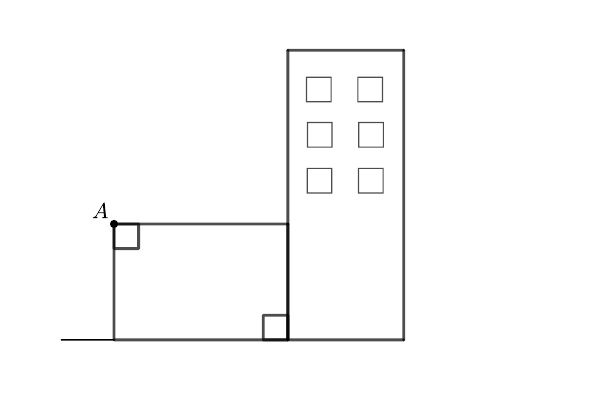
\includegraphics[width=0.55\textwidth]{fig_sel3.png}
\end{center}

\begin{teo}
\textbf{Definición de tangente en un triángulo rectángulo:} $\tan\theta=\dfrac{\text{cateto opuesto}}{\text{cateto adyacente}}$. \textbf{¿Por qué?} Por semejanza de triángulos: la razón opuesto/adyacente sólo depende del ángulo $\theta$, no del tamaño del triángulo.

\textbf{Valor notable:} $\tan 60^\circ=\sqrt{3}$. Se deduce del triángulo equilátero de lado $2$ partido por una altura: la altura mide $\sqrt{3}$, la mitad de la base mide $1$, así que $\tan 60^\circ=\sqrt{3}/1=\sqrt{3}$.
\end{teo}

\begin{paso}{Paso 1 --- Modelo geométrico}
\textbf{Qué hago:} interpreto el dibujo. $A$ está a altura $2$ m del suelo; del punto $A$ sale una horizontal de $7$ m hasta tocar el edificio; el ángulo de elevación entre esa horizontal y la línea de visión a la cima es $60^\circ$.

Llamo $H$ a la altura del edificio (lo que pide el problema) y $h$ a la altura del edificio \emph{por encima de $A$} (lo que se ``ve'' desde $A$). Entonces
\[
H = h + 2,
\]
porque al edificio le falta sumar los $2$ m que están por debajo del nivel de $A$.

\textbf{¿Por qué se suman los $2$?} Porque la línea horizontal desde $A$ \emph{corta} al edificio en un punto que está a $2$ m del suelo; lo que se calcula con trigonometría es la porción \emph{por encima} de esa horizontal.

\textbf{Trampa clásica:} olvidar sumar los $2$ m (eso conduce a la opción C, distractor diseñado para quien comete ese error).
\end{paso}

\begin{paso}{Paso 2 --- Aplico tangente al triángulo rectángulo}
\textbf{Qué hago:} el triángulo tiene cateto adyacente $=7$ m (horizontal) y cateto opuesto $=h$ (parte alta). Aplico
\[
\tan 60^\circ \;=\; \dfrac{h}{7} \quad\Longrightarrow\quad h \;=\; 7\,\tan 60^\circ \;=\; 7\sqrt{3}.
\]

\textbf{¿De dónde sale $\sqrt{3}$?} Del valor exacto $\tan 60^\circ=\sqrt{3}$ (ver teorema arriba).

\textbf{Interpretación:} ``$7\sqrt{3}$'' es cuánto sube la línea de visión al alejarse $7$ m horizontalmente con pendiente $\tan 60^\circ$.

\textbf{Cuidado:} no confundir $\tan 60^\circ$ con $\tan 30^\circ=\tfrac{\sqrt{3}}{3}$. Si se usara $\tan 30^\circ$ aparecería $\tfrac{7\sqrt{3}}{3}$ (opciones A, B); ése es justamente el error que esos distractores buscan provocar.
\end{paso}

\begin{paso}{Paso 3 --- Sumo los $2$ m de la base}
\textbf{Qué hago:} la altura total del edificio es
\[
H \;=\; h + 2 \;=\; 7\sqrt{3} + 2 \text{ m}.
\]

\textbf{¿Qué tomamos?} La expresión $7\sqrt{3}+2$, opción \textbf{D}.
\end{paso}

\begin{resp}
\textbf{Opción D:} altura del edificio $= 7\sqrt{3}+2$ metros.
\end{resp}

% ---------- 4 ----------
\subsection*{Ejercicio 4 --- Afirmaciones sobre $f(x)=\arctan x$}
\addcontentsline{toc}{subsection}{4. arctan: dominio, rango, monotonía}

\textit{Enunciado verbatim:} ``Considere las siguientes afirmaciones de la función definida en su dominio máximo, con criterio $f(x)=\arctan x$.
\begin{itemize}[label={},leftmargin=2em,topsep=2pt,itemsep=0pt]
  \item I. $f$ es estrictamente decreciente.
  \item II. El dominio máximo de $f$ es $[-1,1]$.
  \item III. El ámbito (o rango) de $f$ es $[0,\pi]$.
\end{itemize}
Se puede asegurar que:
\begin{itemize}[label={},leftmargin=2em,topsep=2pt,itemsep=0pt]
  \item A) Ninguna de las afirmaciones es correcta.
  \item B) Solo la afirmación I es correcta.
  \item C) Solo la afirmación II es correcta.
  \item D) Solo la afirmación III es correcta.
\end{itemize}''

\begin{teo}
\textbf{Función $\arctan$ (definición precisa):} es la inversa de $\tan$ \emph{restringida} a $\bigl(-\tfrac{\pi}{2},\tfrac{\pi}{2}\bigr)$, intervalo donde $\tan$ es biyectiva (continua y estrictamente creciente desde $-\infty$ hasta $+\infty$). Como inversa hereda las siguientes propiedades:

\begin{itemize}[leftmargin=*]
  \item \textbf{Dominio:} $\mathbb{R}$ (porque la imagen de $\tan$ restringida era $\mathbb{R}$).
  \item \textbf{Rango:} $\bigl(-\tfrac{\pi}{2},\tfrac{\pi}{2}\bigr)$ (porque era el dominio restringido de $\tan$).
  \item \textbf{Monotonía:} estrictamente \emph{creciente} (la inversa de una función creciente es creciente).
  \item \textbf{Asíntotas horizontales:} $y=\pm\tfrac{\pi}{2}$.
\end{itemize}

\textbf{¿Por qué la inversa de una función creciente es creciente?} Si $f$ es creciente, $a<b\Rightarrow f(a)<f(b)$; tomando $u=f(a)$, $v=f(b)$ tenemos $u<v$ y $f^{-1}(u)=a<b=f^{-1}(v)$.
\end{teo}

\begin{paso}{Paso 1 --- Evalúo cada afirmación}
\textbf{I. ``$f$ es estrictamente decreciente''.} \textbf{FALSA.} $\arctan$ es estrictamente \emph{creciente} (hereda la monotonía de $\tan$ en $(-\tfrac{\pi}{2},\tfrac{\pi}{2})$).

\textbf{II. ``Dominio máximo $=[-1,1]$''.} \textbf{FALSA.} El dominio de $\arctan$ es \emph{todo} $\mathbb{R}$. El intervalo $[-1,1]$ es el dominio de $\arcsen$ y $\arccos$, \emph{no} de $\arctan$.

\textbf{III. ``Rango $=[0,\pi]$''.} \textbf{FALSA.} El rango de $\arctan$ es el intervalo \emph{abierto} $\bigl(-\tfrac{\pi}{2},\tfrac{\pi}{2}\bigr)$. El intervalo $[0,\pi]$ es el rango de $\arccos$.

\textbf{¿Por qué tantas confusiones?} Porque hay tres arco-funciones y cada una tiene su propio dominio/rango. La tabla de memorización:
\[
\begin{array}{c|c|c}
 & \text{Dominio} & \text{Rango}\\\hline
\arcsen & [-1,1] & [-\tfrac{\pi}{2},\tfrac{\pi}{2}]\\
\arccos & [-1,1] & [0,\pi]\\
\arctan & \mathbb{R} & (-\tfrac{\pi}{2},\tfrac{\pi}{2})
\end{array}
\]

\textbf{Regla mental:} ``$\arctan$ acepta cualquier número pero contesta sólo entre $\pm\tfrac{\pi}{2}$, exclusivos''.

\textbf{¿Qué tomamos?} Ninguna afirmación es verdadera $\Rightarrow$ opción \textbf{A}.
\end{paso}

\begin{resp}
\textbf{Opción A:} Ninguna de las tres afirmaciones es correcta.
\end{resp}

% ---------- 5 ----------
\subsection*{Ejercicio 5 --- Amplitud y periodo desde la gráfica cosenoidal}
\addcontentsline{toc}{subsection}{5. Amplitud y periodo}

\textit{Enunciado verbatim:} ``Considere la gráfica adjunta de un periodo completo de una curva cosenoidal. Con certeza, se puede asegurar que su amplitud $A$ y su periodo $P$ son
\begin{itemize}[label={},leftmargin=2em,topsep=2pt,itemsep=0pt]
  \item A) $A=6$ y $P=\dfrac{2\pi}{3}$
  \item B) $A=6$ y $P=\dfrac{\pi}{3}$
  \item C) $A=3$ y $P=\dfrac{2\pi}{3}$
  \item D) $A=3$ y $P=\dfrac{\pi}{3}$
\end{itemize}''

\begin{center}
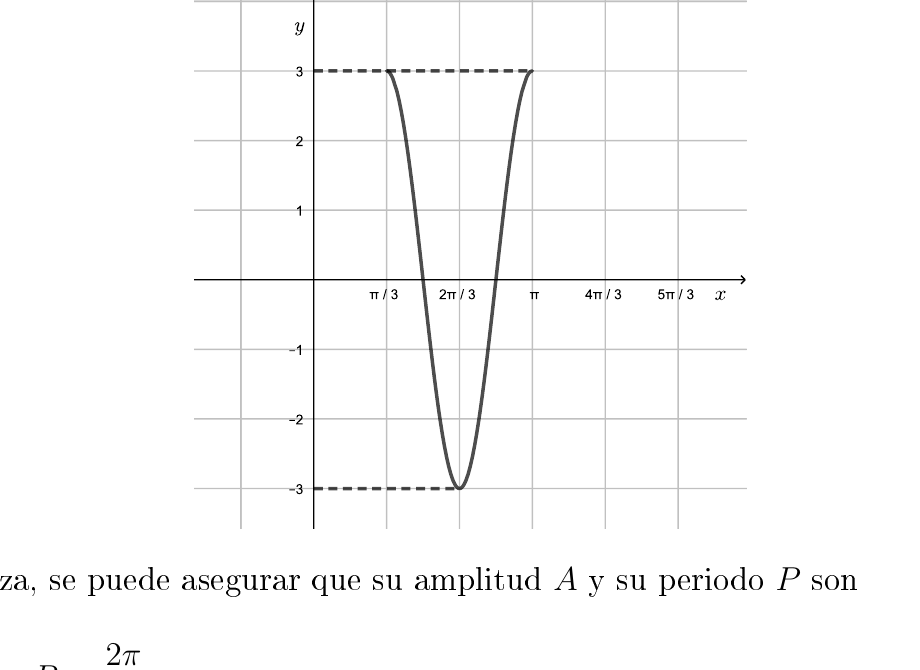
\includegraphics[width=0.7\textwidth]{fig_sel5.png}
\end{center}

\begin{teo}
\textbf{Función cosenoidal genérica:} $y=A\cos(Bx+C)+D$.
\begin{itemize}[leftmargin=*]
  \item \textbf{Amplitud:} $A=\dfrac{y_{\max}-y_{\min}}{2}$. \textbf{¿Por qué la mitad?} Porque $A$ mide la distancia del valor medio al pico, no el ``ancho total'' de oscilación.
  \item \textbf{Periodo:} $P=\dfrac{2\pi}{|B|}$. Es la distancia horizontal entre dos puntos consecutivos en que la curva repite su patrón (por ejemplo, máximo a máximo, o mínimo a mínimo).
\end{itemize}
\end{teo}

\begin{paso}{Paso 1 --- Leo amplitud}
\textbf{Qué hago:} de la gráfica, $y_{\max}=3$ y $y_{\min}=-3$. Entonces
\[
A \;=\; \dfrac{3-(-3)}{2} \;=\; \dfrac{6}{2} \;=\; 3.
\]

\textbf{Trampa:} ``$A=6$'' es el \emph{rango total} (max menos min), no la amplitud. Las opciones A y B son distractores para quien confunde estas dos cantidades.

\textbf{Regla mental:} ``Amplitud = media diferencia entre cresta y valle, NUNCA la diferencia entera''.
\end{paso}

\begin{paso}{Paso 2 --- Leo periodo}
\textbf{Qué hago:} observo dos eventos repetidos. La curva alcanza el valor máximo $y=3$ a lo largo de un tramo dashed que termina en $x=\tfrac{2\pi}{3}$, baja al mínimo $y=-3$ en $x=\pi$, y vuelve al máximo $y=3$ en $x=\tfrac{4\pi}{3}$ (donde reinicia el tramo dashed superior).

Distancia ``máximo a máximo'' $\Rightarrow$ un periodo completo:
\[
P \;=\; \tfrac{4\pi}{3} - \tfrac{2\pi}{3} \;=\; \tfrac{2\pi}{3}.
\]

\textbf{Verificación alternativa:} de mínimo a mínimo siguiente tendría que dar lo mismo, $\tfrac{2\pi}{3}$. La distancia ``máximo a mínimo'' (mitad del periodo) sería $\tfrac{\pi}{3}$, que es exactamente lo que aparece como \emph{distractor} en B y D.

\textbf{Cuidado:} no confundir ``mitad del periodo'' con ``periodo''. La gráfica muestra el descenso de máximo a mínimo en $\tfrac{\pi}{3}$ unidades; pero el patrón completo requiere también volver al máximo, así que el periodo verdadero es $\tfrac{2\pi}{3}$.

\textbf{Regla mental:} ``Periodo = lo que tarda en \emph{repetirse}, no en \emph{subir o bajar} una vez''.

\textbf{¿Qué tomamos?} $A=3$, $P=\tfrac{2\pi}{3}$ $\Rightarrow$ opción \textbf{C}.
\end{paso}

\begin{resp}
\textbf{Opción C:} $A=3$, $P=\dfrac{2\pi}{3}$.
\end{resp}

% ---------- 6 ----------
\subsection*{Ejercicio 6 --- Proposiciones sobre $f:\bigl(\tfrac{\pi}{2},\tfrac{3\pi}{2}\bigr)\to\mathbb{R}$, $f(x)=\tan x$}
\addcontentsline{toc}{subsection}{6. Tan en (pi/2, 3pi/2)}

\textit{Enunciado verbatim:} ``Considere las siguientes proposiciones sobre la función $f:\left]\dfrac{\pi}{2},\dfrac{3\pi}{2}\right[\to\mathbb{R}$ con $f(x)=\tan x$:
\begin{itemize}[label={},leftmargin=2em,topsep=2pt,itemsep=0pt]
  \item I. $f$ es creciente.
  \item II. El ámbito de $f$ es $\mathbb{R}$.
  \item III. $f$ contiene el punto $(\pi,0)$.
\end{itemize}
De ellas, ¿cuáles son verdaderas?
\begin{itemize}[label={},leftmargin=2em,topsep=2pt,itemsep=0pt]
  \item A) Todas
  \item B) Solo I y II
  \item C) Solo I y III
  \item D) Solo II y III
\end{itemize}''

\begin{teo}
\textbf{Tangente:} $\tan x=\dfrac{\sen x}{\cos x}$. Tiene asíntotas verticales donde $\cos x=0$, es decir, $x=\tfrac{\pi}{2}+k\pi$, $k\in\mathbb{Z}$. Entre dos asíntotas consecutivas $\tan$ es continua, estrictamente creciente y su imagen es todo $\mathbb{R}$.

\textbf{¿Por qué creciente entre asíntotas?} La derivada $\tan'x=\sec^2 x>0$ siempre que esté definida.
\end{teo}

\begin{paso}{Paso 1 --- Analizo el dominio $\left(\tfrac{\pi}{2},\tfrac{3\pi}{2}\right)$}
\textbf{Qué hago:} verifico si hay alguna asíntota \emph{dentro} del intervalo abierto.

Las asíntotas de $\tan$ son $\tfrac{\pi}{2},\tfrac{3\pi}{2},\tfrac{5\pi}{2},\ldots$ y sus negativos. Tanto $\tfrac{\pi}{2}$ como $\tfrac{3\pi}{2}$ son los \emph{extremos} del intervalo, y como el intervalo es \emph{abierto}, esos puntos no pertenecen al dominio. En el \emph{interior} $\left(\tfrac{\pi}{2},\tfrac{3\pi}{2}\right)$ no hay otra asíntota, así que $\tan$ es continua y derivable en todo el intervalo.

\textbf{Interpretación:} el intervalo es exactamente \emph{una rama completa} de la tangente (entre dos asíntotas consecutivas).

\textbf{Regla mental:} ``Si el intervalo cae entre dos asíntotas consecutivas y las excluye, $\tan$ se comporta ahí como una sola rama: $-\infty\to+\infty$, creciente''.
\end{paso}

\begin{paso}{Paso 2 --- Evalúo las tres afirmaciones}
\textbf{I. $f$ creciente.} \textbf{VERDADERA.} En cada rama de $\tan$, $\tan'x=\sec^2 x>0$, luego es estrictamente creciente. En particular en $\left(\tfrac{\pi}{2},\tfrac{3\pi}{2}\right)$.

\textbf{II. Ámbito $=\mathbb{R}$.} \textbf{VERDADERA.} Cerca de $\tfrac{\pi}{2}^+$ se tiene $\tan x\to -\infty$ (porque $\cos x\to 0^-$ y $\sen x\to 1^+$, cociente positivo sobre infinitesimal negativo $\to -\infty$). Cerca de $\tfrac{3\pi}{2}^-$, $\cos x\to 0^+$ y $\sen x\to -1$, así que $\tan x\to -\infty/0^+\to -\infty$\ldots un momento, hagamos esto con cuidado.

\smallskip
\textbf{Detalle de los límites (importante):}
\begin{itemize}[leftmargin=*]
  \item Cuando $x\to (\tfrac{\pi}{2})^+$: $\sen x\to 1$, $\cos x\to 0^-$ (porque pasamos a QII donde $\cos<0$). Cociente $\dfrac{1}{0^-}=-\infty$.
  \item Cuando $x\to (\tfrac{3\pi}{2})^-$: $\sen x\to -1$, $\cos x\to 0^-$ (todavía estamos en QIII, donde $\cos<0$). Cociente $\dfrac{-1}{0^-}=+\infty$.
\end{itemize}
Como $f$ es continua creciente que va de $-\infty$ a $+\infty$ en el intervalo, por el teorema del valor intermedio su imagen es todo $\mathbb{R}$.

\textbf{III. Contiene $(\pi,0)$.} \textbf{VERDADERA.} $\pi$ está dentro de $\left(\tfrac{\pi}{2},\tfrac{3\pi}{2}\right)$ y $\tan\pi=\dfrac{\sen\pi}{\cos\pi}=\dfrac{0}{-1}=0$. Por lo tanto el punto $(\pi,0)$ pertenece a la gráfica.

\textbf{Regla mental:} ``$\tan(k\pi)=0$ siempre que $k$ sea entero''.

\textbf{¿Qué tomamos?} I, II y III son verdaderas $\Rightarrow$ opción \textbf{A}.
\end{paso}

\begin{resp}
\textbf{Opción A:} Todas las proposiciones son verdaderas.
\end{resp}

\clearpage
% ============================================================
\section*{Desarrollo}
\addcontentsline{toc}{section}{Desarrollo}

% ---------- D1 ----------
\subsection*{Ejercicio 1 --- $h(x)=\ln(-x+12)+3$: dominio e inversa}
\addcontentsline{toc}{subsection}{D1. Dominio e inversa de h}

\textit{Enunciado verbatim:} ``Considere la función $h:D_h\to\mathbb{R}$, $h(x)=\ln(-x+12)+3$.
a) Determine el dominio de $h$. \textbf{1 punto}
b) Sabiendo que $h$ posee inversa, determine el criterio de $h^{-1}$. \textbf{2 puntos}''

\begin{teo}
\textbf{Dominio de $\ln$:} $\ln u$ está definido $\Leftrightarrow u>0$. \textbf{¿Por qué estrictamente $>0$?} Porque $\ln$ es la inversa de $e^x$, cuya imagen es $(0,\infty)$. El logaritmo no acepta $0$ ni negativos.

\textbf{Método para hallar inversa:} (1) escribir $y=h(x)$; (2) despejar $x$ en términos de $y$; (3) intercambiar nombres: la fórmula resultante es $h^{-1}(x)$. \textbf{¿Por qué funciona?} Porque $y=h(x)\Leftrightarrow x=h^{-1}(y)$ por definición de inversa.
\end{teo}

\begin{paso}{Paso 1 (parte a) --- Dominio: imponer argumento del log $>0$}
\textbf{Qué hago:} exijo $-x+12>0$.

\[
-x+12>0 \;\Longleftrightarrow\; -x>-12 \;\Longleftrightarrow\; x<12.
\]

\textbf{¿De dónde sale el cambio de signo?} Al multiplicar (o dividir) una desigualdad por un número \emph{negativo} ($-1$ en este caso, al despejar $x$), la desigualdad se \emph{invierte}: $-x>-12$ se convierte en $x<12$.

\textbf{Cuidado:} esta es la trampa más frecuente. Quien olvida invertir el sentido obtiene $x>12$, que es justamente el complemento del dominio correcto.

\textbf{Interpretación:} $\ln$ ``come'' sólo positivos; el argumento $-x+12$ es positivo precisamente cuando $x$ no excede $12$.

\textbf{¿Qué tomamos?} El conjunto de los reales menores que $12$: $D_h=\,\left]-\infty,12\right[$.
\end{paso}

\begin{resp}
\textbf{(a)} $D_h=\left]-\infty,12\right[$.
\end{resp}

\begin{paso}{Paso 2 (parte b) --- Despejo $x$ en $y=\ln(-x+12)+3$}
\textbf{Qué hago:} aislar primero el logaritmo, luego deshacer con la exponencial.

\textbf{Aislo el log:} resto $3$ a ambos lados.
\[
y-3 \;=\; \ln(-x+12).
\]

\textbf{Deshago el log:} aplico $e^{(\cdot)}$ a ambos lados, usando $e^{\ln u}=u$.
\[
e^{\,y-3} \;=\; -x+12.
\]

\textbf{¿Por qué $e^{\ln u}=u$?} Porque $\ln$ y $e^{(\cdot)}$ son inversas mutuas por definición; componerlas en cualquier orden da la identidad (en su dominio).

\textbf{Despejo $x$:} paso $12$ y multiplico por $-1$.
\[
e^{\,y-3} - 12 \;=\; -x \;\Longleftrightarrow\; x \;=\; 12 - e^{\,y-3}.
\]

\textbf{Intercambio nombres:} la inversa, vista como función de su propio insumo, es
\[
h^{-1}(x) \;=\; 12 - e^{\,x-3}.
\]

\textbf{Interpretación:} la función original toma un $x<12$, calcula ``cuánto le falta a $x$ para llegar a $12$'' (eso es $-x+12$), le toma logaritmo y le suma $3$. La inversa hace lo opuesto: dado $y$ resta $3$, deshace el log con $e$ y vuelve a la posición $12-(\cdot)$.

\textbf{Verificación rápida:} dominio de $h^{-1}$ debería coincidir con rango de $h$. Como $\ln$ alcanza todo $\mathbb{R}$, el rango de $h$ es $\mathbb{R}$; por lo tanto $h^{-1}$ acepta todos los reales, y en efecto $12-e^{x-3}$ está definido para todo $x\in\mathbb{R}$. \checkmark

\textbf{Regla mental:} ``Para invertir un logaritmo: aisla el log, exponencia, despeja''.

\textbf{¿Qué tomamos?} $h^{-1}(x)=12-e^{x-3}$.
\end{paso}

\begin{resp}
\textbf{(b)} $h^{-1}(x)=12-e^{\,x-3}$.
\end{resp}

% ---------- D2 ----------
\subsection*{Ejercicio 2 --- Resuelva $25^x-5^x-5^x=15$}
\addcontentsline{toc}{subsection}{D2. Ecuación exponencial}

\textit{Enunciado verbatim:} ``Resuelva la ecuación $25^x-5^x-5^x=15$. \textbf{3 puntos}''

\begin{teo}
\textbf{Reescritura de bases:} $25=5^2$, luego $25^x=(5^2)^x=5^{2x}$ por la regla $(a^m)^n=a^{mn}$. \textbf{¿Por qué $(a^m)^n=a^{mn}$?} Porque elevar a la $n$ significa multiplicar la base por sí misma $n$ veces; cada copia contribuye $m$ factores de $a$, total $mn$ factores.

\textbf{Cambio de variable estrella en ecuaciones exponenciales:} si toda la ecuación se puede escribir en términos de $a^x$ y $a^{2x}=(a^x)^2$, sustituye $y=a^x$ para obtener una cuadrática en $y$.
\end{teo}

\begin{paso}{Paso 1 --- Reescribir $25^x$ como $5^{2x}$ y juntar los $5^x$}
\textbf{Qué hago:}
\[
25^x-5^x-5^x \;=\; 15 \;\Longleftrightarrow\; 5^{2x}-2\cdot 5^x-15 \;=\; 0.
\]

\textbf{¿De dónde sale el $-2\cdot 5^x$?} De sumar términos semejantes: $-5^x-5^x=-(1+1)\cdot 5^x=-2\cdot 5^x$ (distribución inversa).

\textbf{¿De dónde sale el $-15$?} De pasar el $15$ del lado derecho al izquierdo cambiándole el signo.

\textbf{Interpretación:} la ecuación es ``cuadrática disfrazada'' en la variable $5^x$. El truco es ver $5^{2x}=(5^x)^2$.

\textbf{Regla mental:} ``Si veo $a^{2x}$ y $a^x$ juntos en una ecuación, sustituyo $y=a^x$ y obtengo cuadrática''.
\end{paso}

\begin{paso}{Paso 2 --- Cambio de variable $y=5^x$}
\textbf{Qué hago:} sustituir $y=5^x$ (de modo que $y^2=5^{2x}$).
\[
y^2 - 2y - 15 \;=\; 0.
\]

\textbf{Factorizo} buscando dos números que sumen $-2$ y multipliquen $-15$: son $-5$ y $+3$.
\[
(y-5)(y+3) \;=\; 0 \;\Longrightarrow\; y=5 \;\;\vee\;\; y=-3.
\]

\textbf{Verificación:} $(y-5)(y+3)=y^2+3y-5y-15=y^2-2y-15$. \checkmark

\textbf{Regla mental:} ``trinomio $y^2+by+c$: dos números que sumen $b$ y multipliquen $c$''.
\end{paso}

\begin{paso}{Paso 3 --- Vuelvo a la variable $x$ y descarto soluciones imposibles}
\textbf{Caso $y=5$:} $5^x=5=5^1\Rightarrow x=1$. (Inyectividad de la exponencial: $a^u=a^v\Rightarrow u=v$ cuando $a>0,a\neq 1$.)

\textbf{Caso $y=-3$:} $5^x=-3$. \textbf{Imposible:} la función exponencial $5^x$ es siempre positiva (su rango es $(0,\infty)$). Una potencia de base positiva nunca puede dar resultado negativo. Esta solución se descarta.

\textbf{¿Por qué $5^x>0$ siempre?} Porque $5^x=e^{x\ln 5}$ y la exponencial $e^{(\cdot)}$ tiene imagen estrictamente positiva.

\textbf{Cuidado:} no olvidar este filtro. Olvidar descartar $y=-3$ no afecta la respuesta final aquí, pero en otros problemas haría que escribieras una solución espuria.

\textbf{Regla mental:} ``$a^x>0$ siempre; si la cuadrática manda valor negativo o $0$, lo descartas''.

\textbf{¿Qué tomamos?} Sólo $x=1$.
\end{paso}

\begin{resp}
$S=\{1\}$.
\end{resp}

% ---------- D3 ----------
\subsection*{Ejercicio 3 --- Verifique la identidad $\dfrac{1}{1-\sen\theta}-\dfrac{1}{1+\sen\theta}=\dfrac{2\tan\theta}{\cos\theta}$}
\addcontentsline{toc}{subsection}{D3. Identidad trigonométrica}

\textit{Enunciado verbatim:} ``Verifique la siguiente identidad trigonométrica.
$\dfrac{1}{1-\sen\theta}-\dfrac{1}{1+\sen\theta}=\dfrac{2\tan\theta}{\cos\theta}$. \textbf{3 puntos}''

\begin{teo}
\textbf{Estrategia general:} se trabaja \emph{un solo lado} (típicamente el más complicado) y se transforma hasta que coincida con el otro. \textbf{¿Por qué un solo lado?} Porque trabajar ambos lados a la vez corre el riesgo de multiplicar por cero o introducir pasos no reversibles.

\textbf{Identidades pivote:}
\begin{itemize}[leftmargin=*]
  \item Pitagórica: $\sen^2\theta+\cos^2\theta=1\Rightarrow 1-\sen^2\theta=\cos^2\theta$.
  \item Diferencia de cuadrados: $(a-b)(a+b)=a^2-b^2$.
  \item Definición: $\tan\theta=\dfrac{\sen\theta}{\cos\theta}$.
\end{itemize}
\end{teo}

\begin{paso}{Paso 1 --- Común denominador en el lado izquierdo}
\textbf{Qué hago:} las dos fracciones del LI tienen denominadores $1-\sen\theta$ y $1+\sen\theta$. El común denominador es su producto $(1-\sen\theta)(1+\sen\theta)$.

\[
\text{LI} \;=\; \dfrac{1}{1-\sen\theta}-\dfrac{1}{1+\sen\theta}
\;=\; \dfrac{(1+\sen\theta)-(1-\sen\theta)}{(1-\sen\theta)(1+\sen\theta)}.
\]

\textbf{¿De dónde sale el numerador?} ``Cruzas'' los numeradores con los denominadores opuestos: el primero gana el factor $(1+\sen\theta)$, el segundo gana $(1-\sen\theta)$. El signo $-$ de la resta se mantiene.

\textbf{Cuidado:} mantener los paréntesis del segundo numerador es vital; sin ellos el signo $-$ no distribuye correctamente.

\textbf{Regla mental:} ``$\dfrac{A}{B}-\dfrac{C}{D}=\dfrac{AD-BC}{BD}$''.
\end{paso}

\begin{paso}{Paso 2 --- Simplifico numerador y denominador con diferencia de cuadrados}
\textbf{Numerador:} $(1+\sen\theta)-(1-\sen\theta)=1+\sen\theta-1+\sen\theta=2\sen\theta$.

\textbf{Denominador:} $(1-\sen\theta)(1+\sen\theta)=1^2-(\sen\theta)^2=1-\sen^2\theta$, por la identidad diferencia de cuadrados $(a-b)(a+b)=a^2-b^2$.

\[
\text{LI} \;=\; \dfrac{2\sen\theta}{1-\sen^2\theta}.
\]

\textbf{¿Por qué la diferencia de cuadrados?} Porque $(1-\sen\theta)$ y $(1+\sen\theta)$ son conjugados; su producto siempre da ``primero al cuadrado menos segundo al cuadrado''.

\textbf{Regla mental:} ``conjugados $\Rightarrow$ producto = diferencia de cuadrados''.
\end{paso}

\begin{paso}{Paso 3 --- Reemplazo $1-\sen^2\theta$ por $\cos^2\theta$ (pitagórica)}
\textbf{Qué hago:} de $\sen^2\theta+\cos^2\theta=1$ despejo $1-\sen^2\theta=\cos^2\theta$.
\[
\text{LI} \;=\; \dfrac{2\sen\theta}{\cos^2\theta}.
\]

\textbf{Interpretación:} hemos reemplazado una expresión ``mixta'' (con seno) por otra puramente coseno; esto encamina el lado izquierdo hacia $\dfrac{\tan}{\cos}$ del lado derecho.
\end{paso}

\begin{paso}{Paso 4 --- Separo $\cos^2\theta$ y armo la tangente}
\textbf{Qué hago:} parto el denominador en $\cos\theta\cdot\cos\theta$ para emparejar uno con $\sen\theta$ y formar $\tan\theta$.
\[
\dfrac{2\sen\theta}{\cos^2\theta}
\;=\; 2\cdot\dfrac{\sen\theta}{\cos\theta}\cdot\dfrac{1}{\cos\theta}
\;=\; 2\tan\theta\cdot\dfrac{1}{\cos\theta}
\;=\; \dfrac{2\tan\theta}{\cos\theta}
\;=\;\text{LD}. \quad\blacksquare
\]

\textbf{¿De dónde sale $\dfrac{\sen\theta}{\cos\theta}=\tan\theta$?} De la definición misma de la tangente.

\textbf{Cuidado:} cuidar las restricciones implícitas. Para que el proceso sea válido se requiere $1\pm\sen\theta\neq 0$ y $\cos\theta\neq 0$, es decir $\theta\neq\tfrac{\pi}{2}+k\pi$. Estas restricciones ya vienen heredadas del lado izquierdo y del derecho.

\textbf{Regla mental:} ``Para una identidad $\sen$/$\cos$/$\tan$: convierte todo a $\sen$ y $\cos$, simplifica, vuelve a re-armar tangentes al final''.
\end{paso}

\begin{resp}
Identidad verificada: $\;\dfrac{1}{1-\sen\theta}-\dfrac{1}{1+\sen\theta}=\dfrac{2\tan\theta}{\cos\theta}$, con $\theta\neq\tfrac{\pi}{2}+k\pi$, $k\in\mathbb{Z}$.
\end{resp}

% ---------- D4 ----------
\subsection*{Ejercicio 4 --- $2\sen x\,\tan x-\tan x=0$ en $[0,2\pi[$}
\addcontentsline{toc}{subsection}{D4. Ecuación trigonométrica con factorización}

\textit{Enunciado verbatim:} ``Determine el conjunto solución de la ecuación $2\sen x\,\tan x-\tan x=0$, $x\in[0,2\pi[$. \textbf{4 puntos}''

\begin{teo}
\textbf{Factor común:} si dos términos comparten un factor, sácalo: $ab\pm ac=a(b\pm c)$. \textbf{¿Por qué?} Por distributividad de la multiplicación sobre la suma, leída al revés.

\textbf{Ley del producto cero:} en $\mathbb{R}$, $u\cdot v=0\Leftrightarrow u=0\,\lor\, v=0$. \textbf{¿Por qué?} Porque $\mathbb{R}$ es un cuerpo y, por tanto, dominio íntegro: no tiene divisores de cero.

\textbf{Ceros notables:}
\begin{itemize}[leftmargin=*]
  \item $\sen x=\tfrac{1}{2}\Rightarrow x=\tfrac{\pi}{6}+2k\pi$ o $x=\tfrac{5\pi}{6}+2k\pi$ (ángulos de referencia en QI y QII donde el seno vale $+\tfrac{1}{2}$).
  \item $\tan x=0\Leftrightarrow \sen x=0$ (con $\cos x\neq 0$) $\Leftrightarrow x=k\pi$.
\end{itemize}
\end{teo}

\begin{paso}{Paso 1 --- Factor común $\tan x$}
\textbf{Qué hago:} ambos términos contienen $\tan x$.
\[
2\sen x\,\tan x-\tan x \;=\; \tan x\,(2\sen x-1) \;=\; 0.
\]

\textbf{¿De dónde sale el ``$-1$'' del paréntesis?} El término ``$-\tan x$'' es ``$-1\cdot\tan x$''; al extraer $\tan x$ queda el ``$-1$'' dentro.

\textbf{Trampa #1 (clásica):} \emph{nunca} dividir entre $\tan x$ para ``cancelar''. Si $\tan x=0$, dividir entre cero borra soluciones legítimas. Por eso \textbf{se factoriza, no se cancela}.

\textbf{Regla mental:} ``Factoriza siempre; cancelar es traicionero''.
\end{paso}

\begin{paso}{Paso 2 --- Aplico ley del producto cero}
\[
\tan x = 0 \quad\lor\quad 2\sen x-1=0 \;\Longleftrightarrow\; \sen x=\tfrac{1}{2}.
\]

\textbf{Interpretación:} cada factor independientemente puede hacer cero el producto; tratamos cada caso por separado y unimos los conjuntos solución.
\end{paso}

\begin{paso}{Paso 3 --- Caso $\tan x=0$ en $[0,2\pi[$}
\textbf{Qué hago:} $\tan x=0\Leftrightarrow \sen x=0$ (con $\cos x\neq 0$, lo cual automáticamente se cumple cuando $\sen x=0$ porque $\sen^2+\cos^2=1$ implica $\cos x=\pm 1\neq 0$).

\textbf{¿Dónde se anula $\sen$ en $[0,2\pi[$?} En $x=0$ y $x=\pi$ (no incluimos $2\pi$ porque el intervalo es semi-abierto a la derecha).

\textbf{¿Qué tomamos?} $x=0$, $x=\pi$.

\textbf{Regla mental:} ``$\sen$ se anula en cada múltiplo entero de $\pi$''.
\end{paso}

\begin{paso}{Paso 4 --- Caso $\sen x=\tfrac{1}{2}$ en $[0,2\pi[$}
\textbf{Qué hago:} el seno vale $+\tfrac{1}{2}$ con ángulo de referencia $\tfrac{\pi}{6}$ (porque $\sen(\tfrac{\pi}{6})=\tfrac{1}{2}$ es valor notable). El seno es positivo en QI y QII.

\textbf{En QI:} $x=\tfrac{\pi}{6}$.

\textbf{En QII:} $x=\pi-\tfrac{\pi}{6}=\tfrac{6\pi-\pi}{6}=\tfrac{5\pi}{6}$. \textbf{¿Por qué $\pi-\theta_{\text{ref}}$?} Porque el seno tiene la simetría $\sen(\pi-\theta)=\sen\theta$ (refleja respecto al eje $y$ en la circunferencia).

\textbf{¿Qué tomamos?} $x=\tfrac{\pi}{6}$, $x=\tfrac{5\pi}{6}$.

\textbf{Regla mental:} ``$\sen=\tfrac{1}{2}\Rightarrow$ ángulos de $30^\circ$ y $150^\circ$''.
\end{paso}

\begin{paso}{Paso 5 --- Reúno las cuatro soluciones}
\[
S \;=\; \left\{\,0,\;\dfrac{\pi}{6},\;\dfrac{5\pi}{6},\;\pi\,\right\}.
\]

\textbf{Verificación rápida ($x=\tfrac{\pi}{6}$):} $\tan\tfrac{\pi}{6}=\tfrac{1}{\sqrt{3}}\neq 0$, pero $2\sen\tfrac{\pi}{6}-1=2\cdot\tfrac{1}{2}-1=0$. Producto $=0$. \checkmark

\textbf{Verificación rápida ($x=\pi$):} $\tan\pi=0$. Producto $=0\cdot(\ldots)=0$. \checkmark
\end{paso}

\begin{resp}
$S=\left\{0,\;\dfrac{\pi}{6},\;\dfrac{5\pi}{6},\;\pi\right\}$.
\end{resp}

% ---------- D5 ----------
\subsection*{Ejercicio 5 --- Dos caminantes, ángulo $50^\circ$, ley de cosenos}
\addcontentsline{toc}{subsection}{D5. Ley de cosenos}

\textit{Enunciado verbatim:} ``Dos personas salen simultáneamente desde un mismo punto con rutas aproximadamente rectilíneas y sobre un terreno plano, que forman un ángulo de $50^\circ$ entre ellas. Si al transcurrir una hora la primera persona ha recorrido $5$ km y entre ellas hay una distancia de $12$ km, ¿qué distancia aproximada ha recorrido la segunda persona? \textbf{3 puntos}''

\begin{center}
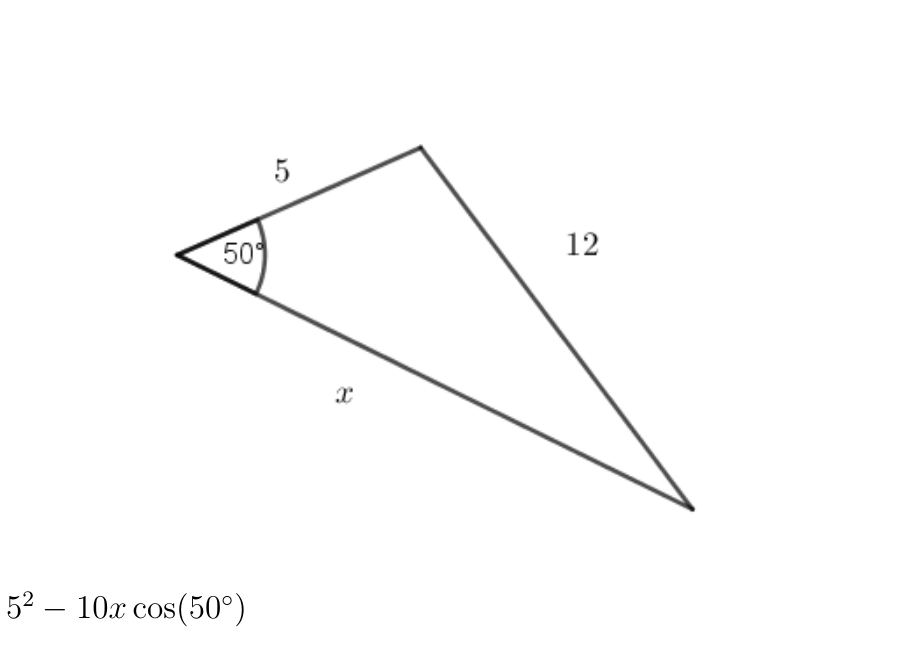
\includegraphics[width=0.55\textwidth]{fig_des5.png}
\end{center}

\begin{teo}
\textbf{Ley de cosenos:} en un triángulo de lados $a,b,c$ y ángulo $C$ \emph{opuesto} al lado $c$,
\[
c^2 \;=\; a^2+b^2-2ab\cos C.
\]
Generaliza el teorema de Pitágoras (que se recupera con $C=90^\circ\Rightarrow \cos C=0$).

\textbf{¿Cuándo usarla?} Cuando conoces ``\textit{lado-ángulo-lado}'' (dos lados y el ángulo entre ellos) y buscas el tercer lado, o conoces los tres lados y buscas un ángulo.
\end{teo}

\begin{paso}{Paso 1 --- Identifico el triángulo y nombro los datos}
\textbf{Qué hago:} dibujo (ya provisto en el enunciado). Llamo:
\begin{itemize}[leftmargin=*]
  \item $a=5$ km: lado conocido (primera persona).
  \item $x$ km: lado desconocido (segunda persona).
  \item $c=12$ km: lado opuesto al ángulo dado de $50^\circ$ (distancia entre las dos personas, frente al vértice donde se forman las rutas).
  \item Ángulo entre los lados $a$ y $x$: $C=50^\circ$.
\end{itemize}

\textbf{¿Por qué $12$ es el lado opuesto al ángulo $50^\circ$?} Porque las personas \emph{parten} del mismo punto (donde está el ángulo de $50^\circ$); las distancias caminadas son los \emph{lados} que parten del ángulo, y la distancia \emph{entre ellas} es el lado al frente.

\textbf{Regla mental:} ``El lado opuesto al ángulo es el que NO toca al vértice del ángulo''.
\end{paso}

\begin{paso}{Paso 2 --- Aplico ley de cosenos}
\textbf{Qué hago:} sustituyo en $c^2=a^2+x^2-2ax\cos C$ con $c=12$, $a=5$, $C=50^\circ$.
\[
12^2 \;=\; 5^2+x^2-2\cdot 5\cdot x\cdot\cos 50^\circ
\;\Longleftrightarrow\; 144 \;=\; 25+x^2-10x\cos 50^\circ.
\]

\textbf{Paso a forma estándar de cuadrática:} llevo todo a un lado.
\[
x^2 - 10\cos 50^\circ\cdot x + 25 - 144 \;=\; 0 \;\Longleftrightarrow\; x^2 - 10\cos 50^\circ\cdot x - 119 \;=\; 0.
\]

\textbf{¿De dónde sale $-119$?} De $25-144=-119$ al consolidar las constantes.

\textbf{Cuidado:} preservar el signo del término $-10x\cos 50^\circ$. Si se olvida el signo $-$ se obtiene una ecuación distinta cuya raíz positiva es muy diferente.
\end{paso}

\begin{paso}{Paso 3 --- Resuelvo cuadrática con fórmula general}
\textbf{Qué hago:} aplico $x=\dfrac{-b\pm\sqrt{b^2-4ac}}{2a}$ a $x^2-(10\cos 50^\circ)\,x-119=0$.

Identifico coeficientes: $A=1$, $B=-10\cos 50^\circ$, $C=-119$.

\textbf{Valor numérico:} $\cos 50^\circ\approx 0.6428$, así que $10\cos 50^\circ\approx 6.428$. Por lo tanto $B\approx -6.428$.

\textbf{Discriminante:}
\[
\Delta \;=\; B^2-4AC \;=\; (-6.428)^2 - 4(1)(-119) \;\approx\; 41.32 + 476 \;\approx\; 517.32.
\]
\[
\sqrt{\Delta} \;\approx\; 22.74.
\]

\textbf{Raíces:}
\[
x \;=\; \dfrac{6.428\pm 22.74}{2} \;\Longrightarrow\;
\begin{cases}
x_1 \;\approx\; \dfrac{6.428+22.74}{2} \;\approx\; \dfrac{29.17}{2} \;\approx\; 14.58,\\[6pt]
x_2 \;\approx\; \dfrac{6.428-22.74}{2} \;\approx\; \dfrac{-16.31}{2} \;\approx\; -8.16.
\end{cases}
\]

\textbf{¿De dónde sale el $\pm$?} De extraer raíz cuadrada del discriminante, donde aparecen los dos signos.

\textbf{Interpretación geométrica:} la ecuación cuadrática refleja que, dado un ángulo y dos longitudes (la conocida y la distancia entre ambos), podría haber \emph{dos} triángulos compatibles (configuración ``lado-lado-ángulo''); sin embargo, una distancia debe ser positiva.
\end{paso}

\begin{paso}{Paso 4 --- Filtro físico: descarto raíz negativa}
\textbf{Qué hago:} $x$ representa una distancia \emph{recorrida}, por lo tanto $x>0$. Descarto $x_2\approx -8.16$.

\textbf{¿Por qué descartar?} Porque distancias negativas no tienen sentido físico (no se ``camina negativo''). El modelo cuadrático devuelve la opción extra como artefacto algebraico.

\textbf{¿Qué tomamos?} $x\approx 14.5$ km.

\textbf{Regla mental:} ``Después de la cuadrática, siempre filtra contra el dominio físico/algebraico del problema''.
\end{paso}

\begin{resp}
La segunda persona ha recorrido aproximadamente $\boxed{x\approx 14.5\text{ km}}$.
\end{resp}

\vspace{1em}
\begin{nota}
\textbf{Observación sobre el ejercicio faltante.} El enunciado del examen anuncia ``seis preguntas de desarrollo''. La versión del PDF entregada termina con el ejercicio 5 anterior; no contiene el enunciado del ejercicio 6 de desarrollo, por lo cual no se resuelve. Si el usuario aporta el sexto enunciado, se anexará al solucionario con el mismo nivel de detalle.
\end{nota}

\end{document}
